\chapter{Alguns exemplos de comandos \LaTeX{}}

\section{Bibliografia e Referências}

A documentação do pacote biblatex\index{biblatex} é bastante extensa e explica
os diversos tipos de documento suportados, bem como o significado
de cada campo. Na prática, às vezes é preciso fazer escolhas sobre
o que incluir na descrição de um item bibliográfico e muitas vezes
é mais fácil aprender copiando exemplos já existentes, como estes:

\begin{itemize}
\item @Book: \cite{JW82}.
{\scriptsize\begin{verbatim}
@Book{JW82,
 author   = {Richard A. Johnson and Dean W. Wichern},
 title    = {Applied Multivariate Statistical Analysis},
 publisher= {Prentice-Hall},
 year     = {1983}
}
\end{verbatim}
}

\item @Article: \cite{MenaChalco08}.
{\scriptsize\begin{verbatim}
@Article{MenaChalco08,
 author   = {Jesús P. Mena-Chalco and Helaine Carrer and Yossi Zana and
            Roberto M. Cesar-Jr.},
 title    = {Identification of protein coding regions using the modified
            {G}abor-wavelet transform},
 journal  = {IEEE/ACM Transactions on Computational Biology and Bioinformatics},
 volume   = {5},
 pages    = {198-207},
 year     = {2008},
}
\end{verbatim}
}

\item @InProceedings: \cite{alves03:simi}.
{\scriptsize\begin{verbatim}
@InProceedings{alves03:simi,
 author   = {Carlos E. R. Alves and Edson N. Cáceres and Frank Dehne and
            Siang W. Song},
 title    = {A Parallel Wavefront Algorithm for Efficient Biological
            Sequence Comparison},
 booktitle= {ICCSA '03: The 2003 International Conference on Computational Science
            and its Applications},
 year     = {2003},
 pages    = {249-258},
 month    = May,
 publisher= {Springer-Verlag}
}
\end{verbatim}
}

\item @InCollection: \cite{bobaoglu93:concepts}.
{\scriptsize\begin{verbatim}
@InCollection{bobaoglu93:concepts,
 author   = {Ozalp Babaoglu and Keith Marzullo},
 title    = {Consistent Global States of Distributed Systems: Fundamental Concepts
            and Mechanisms},
 editor   = {Sape Mullender},
 booktitle= {Distributed Systems},
 edition  = {segunda},
 year     = {1993},
 pages    = {55-96}
}
\end{verbatim}
}

\item @Conference: \cite{bronevetsky02}.
{\scriptsize\begin{verbatim}
@Conference{bronevetsky02,
 author   = {Greg Bronevetsky and Daniel Marques and Keshav Pingali and
            Paul Stodghill},
 title    = {Automated application-level checkpointing of {MPI} programs},
 booktitle= {PPoPP '03: Proceedings of the 9th ACM SIGPLAN Symposium on Principles
            and Practice of Parallel Programming},
 year     = {2003},
 pages    = {84-89}
}
\end{verbatim}
}

\item @PhdThesis: \cite{garcia01:PhD}.
{\scriptsize\begin{verbatim}
@PhdThesis{garcia01:PhD,
 author   = {Islene C. Garcia},
 title    = {Visões Progressivas de Computações Distribuídas},
 school   = {Instituto de Computação, Universidade de Campinas, Brasil},
 year     = {2001},
 month    = {Dezembro}
}
\end{verbatim}
}

\item @MastersThesis: \cite{schmidt03:MSc}.
{\scriptsize\begin{verbatim}
@MastersThesis{schmidt03:MSc,
 author   = {Rodrigo M. Schmidt},
 title    = {Coleta de Lixo para Protocolos de \emph{Checkpointing}},
 school   = {Instituto de Computação, Universidade de Campinas, Brasil},
 year     = {2003},
 month    = Oct
}
\end{verbatim}
}

\item @Techreport: \cite{alvisi99:analysisCIC}.
{\scriptsize\begin{verbatim}
@Techreport{alvisi99:analysisCIC,
 author   = {Lorenzo Alvisi and Elmootazbellah Elnozahy and Sriram S. Rao and
            Syed A. Husain and Asanka Del Mel},
 title    = {An Analysis of Comunication-Induced Checkpointing},
 institution= {Department of Computer Science, University of Texas at Austin},
 year     = {1999},
 number   = {TR-99-01},
 address  = {Austin, {USA}}
}
\end{verbatim}
}

\item @Manual: \cite{CORBA:spec}.
{\scriptsize\begin{verbatim}
@Manual{CORBA:spec,
 title    = {{CORBA v3.0 Specification}},
 author   = {{Object Management Group}},
 month    = Jul,
 year     = {2002},
 note     = {{OMG Document 02-06-33}}
}
\end{verbatim}
}

\item @Misc: \cite{gridftp}.
{\scriptsize\begin{verbatim}
@Misc{gridftp,
 author   = {William Allcock},
 title    = {{GridFTP} protocol specification. {Global Grid Forum}
            Recommendation ({GFD}.20)},
 year     = {2003}
}
\end{verbatim}
}

\item @Misc: para referência a artigo online \cite{fowler04:designDead}.
{\scriptsize\begin{verbatim}
@Misc{fowler04:designDead,
 author   = {Martin Fowler},
 title    = {Is Design Dead?},
 year     = {2004},
 month    = May,
 note     = {Último acesso em 30/1/2010},
 howpublished= {\url{http://martinfowler.com/articles/designDead.html}},
}
\end{verbatim}
}

\item @Misc: para referência a página web \cite{FSF:GNU-GPL}.
{\scriptsize\begin{verbatim}
@Misc{FSF:GNU-GPL,
 author   = {Free Software Foundation},
 title    = {GNU general public license},
 note     = {Último acesso em 30/1/2010},
 howpublished= {\url{http://www.gnu.org/copyleft/gpl.html}},
}
\end{verbatim}
}

\end{itemize}

\section{Floats (Tabelas e Figuras)}

Talvez você precise organizar a apresentação da informação na forma de
tabelas\index{Floats}. A Tabela \ref{tab:ficha}, por exemplo, mostra como construir
uma tabela em forma de ficha com o \LaTeX{}.

% Aumenta o espaçamento entre as linhas da tabela (default: 0pt)
\setlength\extrarowheight{4pt}

\begin{table}
\begin{tabular}{|M{0.265}|M{0.073}|M{0.084}|M{0.073}|M{0.073}|M{0.08}|M{0.082}|M{0.067}|}
  \hline
    \textbf{Experimento número:} & \multicolumn{2}{c|}{1} & \multicolumn{4}{c|}{\textbf{Data:}} & jan 2017
  \tabularnewline \hline
    \textbf{Título:} & \multicolumn{7}{c|}{Medições iniciais}
  \tabularnewline \hline
    \textbf{Tipo de experimento:} & \multicolumn{7}{c|}{Levantamento quantitativo}
  \tabularnewline \hline \hline
    \textbf{Locais}          & São Paulo & Rio de Janeiro & Porto Alegre & Recife & Manaus & Brasília & Rio Branco
  \tabularnewline \thickhline
    \textbf{Valores obtidos} & 0.2       & 0.3            & 0.2          & 0.7    & 0.5    & 0.1      & 0.4
  \tabularnewline \hline
\end{tabular}
\caption{Exemplo de tabela similar a uma ficha}
\label{tab:ficha}
\end{table}

% Redefinindo para o valor default
\setlength\extrarowheight{0pt}

Há diversos estilos de tabela possíveis; veja outro exemplo na
Tabela \ref{tab:amino_acidos} e mais outro no Apêndice
\ref{ape:sequencias}.

\begin{table}
\begin{center}
    \begin{tabular}{ccl}
    \rothead{Código} & \rothead{Abreviatura} & \rothead{Nome\\completo} \\ \hline
     \texttt{A}      & Ala                   & Alanina \\
     \texttt{C}      & Cys                   & Cisteína \\
     ...             & ...                   & ... \\
     \texttt{W}      & Trp                   & Tiptofano \\
     \texttt{Y}      & Tyr                   & Tirosina \\ \hline
    \end{tabular}
  \caption{Códigos, abreviaturas e nomes dos aminoácidos.}
  \label{tab:amino_acidos}
\end{center}
\end{table}

Muitos trabalhos acadêmicos incluem figuras; um exemplo é a
Figura~\ref{fig:humanbeta}.\index{Floats}

\begin{figure}
  \centering
  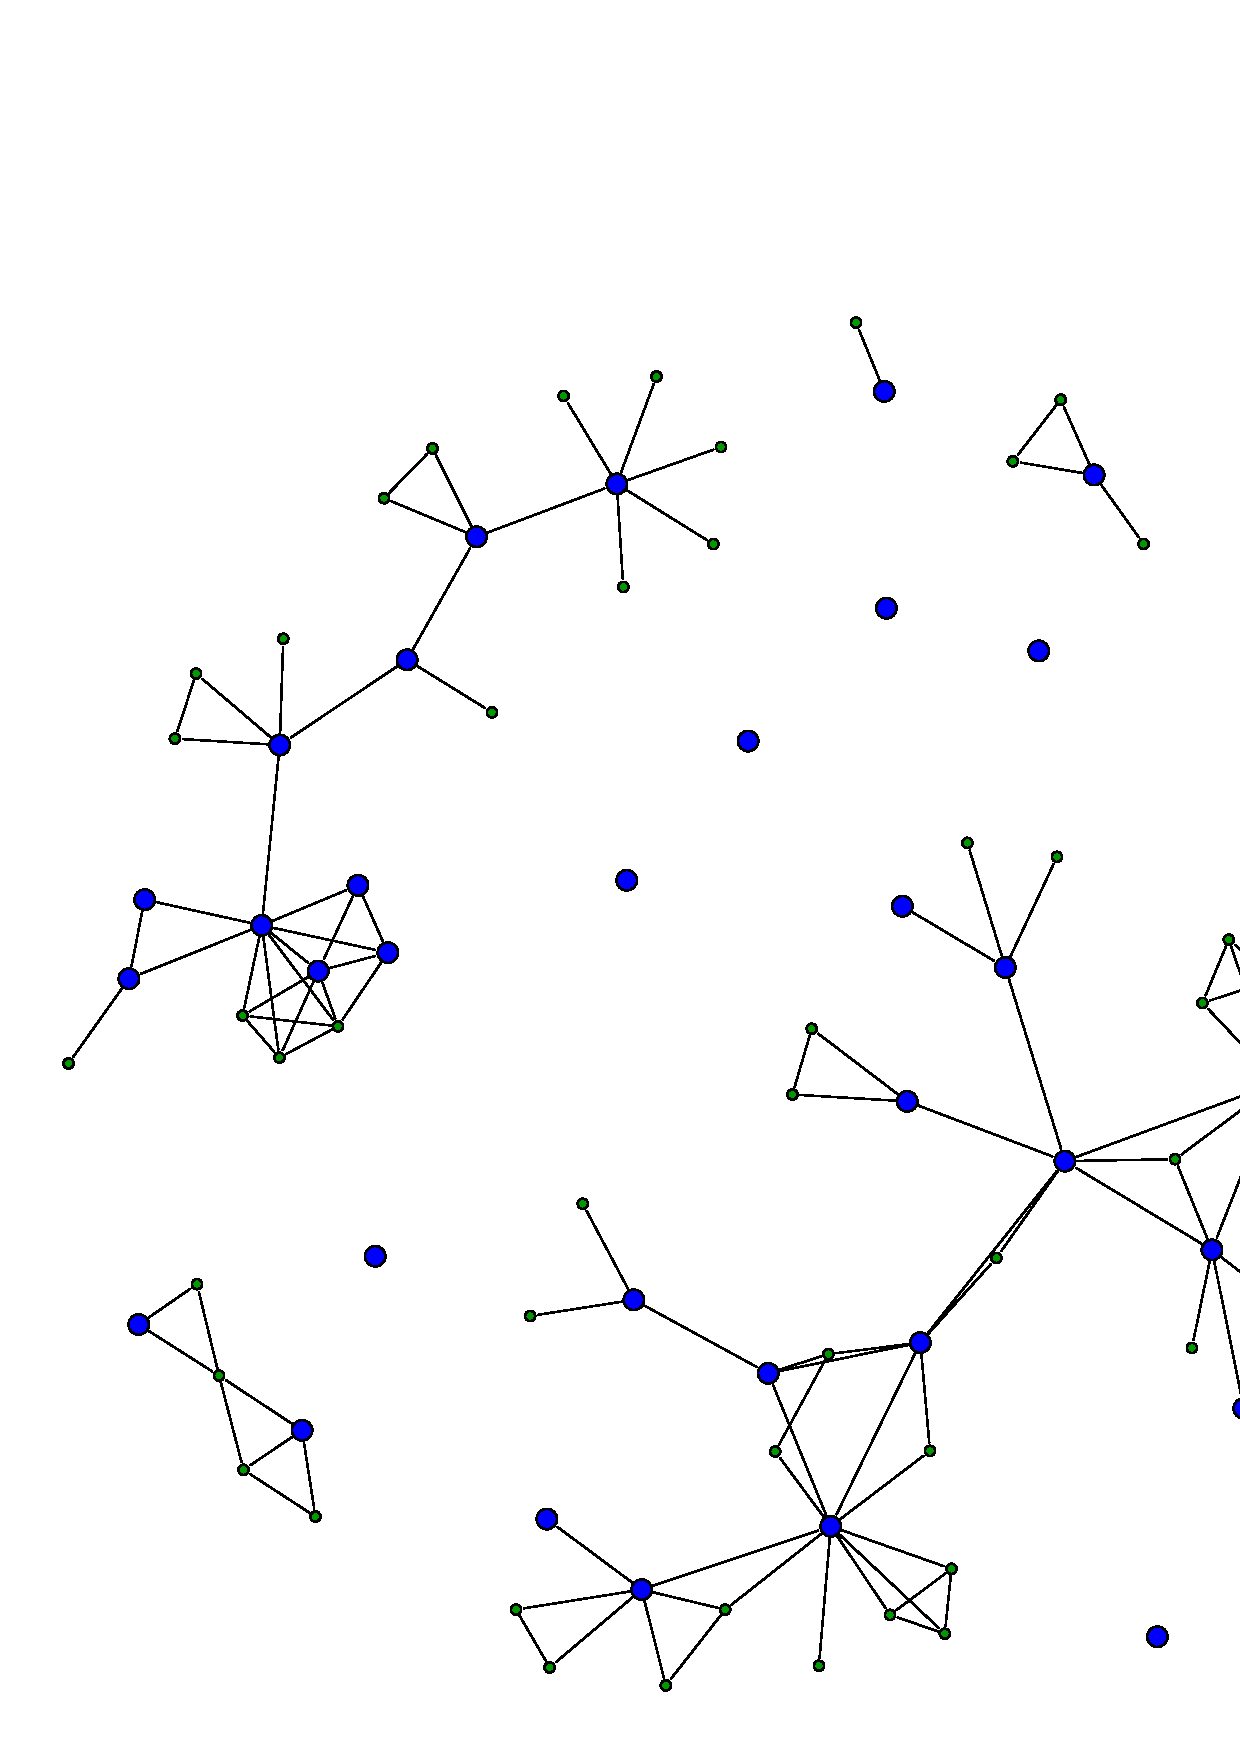
\includegraphics[width=.40\textwidth]{graph}
  \caption{Exemplo de grafo simples}
  \label{fig:humanbeta}
\end{figure}

Pode também ser necessário apresentar trechos de código-fonte, o que pode
ser feito facilmente, como se vê na Figura \ref{fig:java}:\index{Floats}

% Foi utilizado o pacote listing para formatar código fonte
% http://ctan.org/tex-archive/macros/latex/contrib/listings/listings.pdf
% Veja no preambulo do arquivo tese-exemplo.tex os parâmetros de configuração.
\begin{figure}
  \index{Java}
  \centering
  \caption{Exemplo de laço em Java}
  \label{fig:java}
\begin{lstlisting}[language=Java, style=wider]
for(i = 0; i < 20; i++)
{
	// Comentário
	System.out.println("Mensagem...");
}
\end{lstlisting}
\end{figure}

\section{Modo Matemático}

O modo matemático do \LaTeX{} tem sintaxe própria, mas ela não é complicada
e há bastante documentação online a respeito. Um breve exemplo:

\begin{verbatim}
\begin{gather}
\label{eq:2grau}
    ax^2+bx+c=y \quad \forall x \in \mathbb{R}\\
\label{eq:bhaskara}
    y=0 \Leftrightarrow x=\frac{-b \pm \sqrt{\Delta}}{2a}
    \Leftrightarrow x \text{ é raiz da equação}\\
\label{eq:delta}
    \Delta\enspace(\mathit{delta}) = b^2-4ac
\end{gather}

As raízes de uma equação de segundo grau (Equação \ref{eq:2grau})
podem ser encontradas pela fórmula de Bháskara
(Equação \ref{eq:bhaskara}). O valor do discriminante $\Delta$
(Equação \ref{eq:delta}) determina se a equação tem zero, uma ou
duas raízes reais.
\end{verbatim}

Que resulta em:

\begin{gather}
\label{eq:2grau}
	ax^2+bx+c=y \quad \forall x \in \mathbb{R}\\
\label{eq:bhaskara}
    y=0 \Leftrightarrow x=\frac{-b \pm \sqrt{\Delta}}{2a}
    \Leftrightarrow x \text{ é raiz da equação}\\
\label{eq:delta}
    \Delta\enspace(\mathit{delta}) = b^2-4ac
\end{gather}

As raízes de uma equação de segundo grau (Equação \ref{eq:2grau})
podem ser encontradas pela fórmula de Bháskara
(Equação \ref{eq:bhaskara}). O valor do discriminante $\Delta$
(Equação \ref{eq:delta}) determina se a equação tem zero, uma ou
duas raízes reais.
